

\فصل{موتور تشخیص الکترونیکی حروف}

یکی از واحدهای اصلی این برنامک، موتور تشخیص الکترونیکی حروف است. تحقیقی در زمینه محک موتورهای مختلف صورت گرفت. در این فصل به اختصار دو تا از موتورهای مهم را مورد بررسی قرار می‌دهیم:

\قسمت{OCR Google}



\شروع{شکل}[ht]
\begin{center}
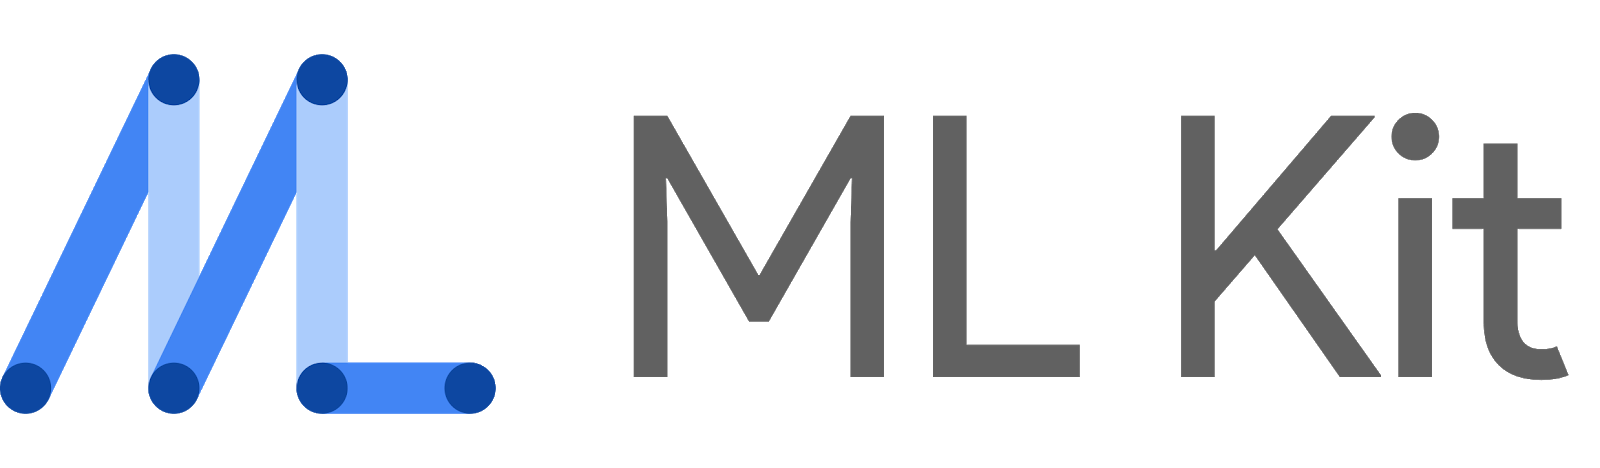
\includegraphics[scale=0.15]{front/template/images/ml-kit.png}
\end{center}
\شرح{موتور تشخیص الکترونیکی حروف Kit ML}
\پایان{شکل}

\شروع{شمارش}

\فقره 
مزیت: مجموعه داده‌هاي آموزش را به صورت برخط درون‌ریزي میکند و در نتیجه
حجم نسخه نصبی برنامه به کمترین مقدار ممکن خود میرسد.

\فقره 
 مزیت: دقت تشخیص حروف در Kit ML شرکت گوگل بالاتر از بقیه موتورهاي
تشخیص الکترونیکی حروف است.

\فقره 
عیب: با توجه به تحریم‌هاي دولت آمریکا علیه کشور ما، این خدمت روي گوشی‌هاي
همراه ایران با خلل روبه‌رو است.
\پایان{شمارش}


\قسمت{Engine OCR Tesseract}

\شروع{شکل}[ht]
\begin{center}
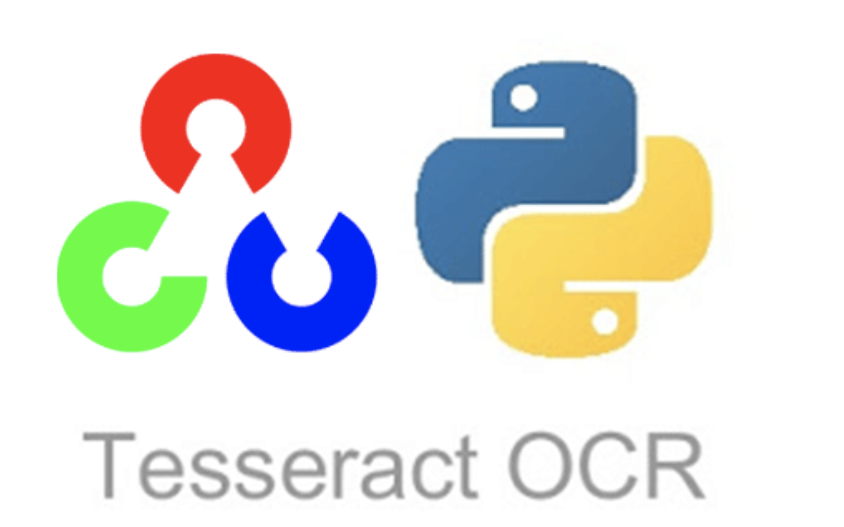
\includegraphics[scale=0.45]{front/template/images/tesseract.png}
\end{center}
\شرح{موتور تشخیص الکترونیکی حروف Tesseract}
\پایان{شکل}


\شروع{شمارش}

\فقره 
مزیت: برنامک می‌تواند به صورت کاملا برون‌خط کار کند و مشکل تحریم را نیز
نخواهیم داشت. 
\فقره 
عیب: براي اینکه سرعت پردازش خوبی داشته باشیم نیاز است تا مجموعه داده‌هاي
آموزش را درون برنامه داشته باشیم که تا ۲۲ مگابایت حجم برنامک را افزایش می‌دهد. 

\پایان{شمارش}


\قسمت{نتیجه محک}


بـا تـوجـه بـه اینکه گـزینه اول دقـت بـالاتـري بـه هـمراه دارد و همچنین بـرنـامک حجـم بسیار کمتري خـواهـد داشـت، مـوتـور تشخیص الکترونیکی گـوگـل را انـتخاب میکنیم. ضـمنا بـا تـوجـه بـه این که این بـرنـامک قـرار اسـت در کشور کانـادا مـورد اسـتفاده قـرار گیرد، مشکل تحـریم را نـخواهیم داشـت. الـبته بـرنـامک بـه صـورتی پیاده سـازي شـده اسـت که بـه راحتی میتـوان گـزینه دوم را مـتصل کرد و در ایران نیز خدمت گرفت.
